\documentclass[../../../../main.tex]{subfiles}

\begin{document}

\section*{1984年 東京大学 理科}

\subsection*{第1問}

[解] $C$ の中心 $D\left(0, \frac{\sqrt{2}}{2}, \frac{\sqrt{2}}{2}\right)$ で, 平面 $z=y$ 上にある.
\[
\begin{cases}
y=z \\
x^2 + \left(y-\frac{\sqrt{2}}{2}\right)^2 + \left(z-\frac{\sqrt{2}}{2}\right)^2 = 1
\end{cases}
\quad \dots \text{①}
\]

$S$ の輪郭上の点 $T(X, Y, 0)$ とする.
\[
\vec{OT} = \begin{pmatrix} 0 \\ 0 \\ 2\sqrt{2} \end{pmatrix} + t \begin{pmatrix} X \\ Y \\ -2\sqrt{2} \end{pmatrix} \quad \dots \text{②}
\]
とおける. ①に代入すると,
\[
\begin{cases}
t Y = (1-t) 2\sqrt{2} \\
(t X)^2 + 2 \left(t Y - \frac{\sqrt{2}}{2}\right)^2 = 1
\end{cases}
\quad \dots \text{③}
\]
第1式から, $t = \frac{2\sqrt{2}}{Y + 2\sqrt{2}}$ ($Y \ge 0$ だから). 第2式から,
\[
\frac{8 X^2}{(Y + 2\sqrt{2})^2} + 2 \left( \frac{2\sqrt{2} Y}{Y + 2\sqrt{2}} - \frac{\sqrt{2}}{2} \right)^2 = 1
\]
\[
8 X^2 + 2 \left( 2\sqrt{2} Y - \frac{\sqrt{2}}{2} Y - 2\sqrt{2} \right)^2 = (Y + 2\sqrt{2})^2
\]
\[
\therefore X^2 + (Y - \sqrt{2})^2 = 2
\]
から, もとめるのは, $x^2 + (y - \sqrt{2})^2 = 2$ である.

\begin{center}
\begin{tikzpicture}[scale=1.2, >=stealth]
  % Axes
  \draw[->] (0,0,0) -- (3,0,0) node[right] {$y$};
  \draw[->] (0,0,0) -- (0,3.5,0) node[above] {$z$};
  \draw[->] (0,0,0) -- (0,0,3) node[below left] {$x$};
  \node[below left] at (0,0,0) {$O$};

  % Point P
  \coordinate (P) at (0,2.8,0);
  \fill (P) circle (1.5pt) node[above right] {$P$};
  \node[left] at (P) {$2\sqrt{2}$};

  % Circle/Region S on xy plane
  \draw[dashed] (0,1.4,0) ellipse (1.2 and 0.4);
  \coordinate (T) at (0.8,0,0);
  \fill (T) circle (1.5pt) node[below] {$T$};

  % Lines from P
  \draw (P) -- (-1.2,0,0);
  \draw (P) -- (1.2,0,0);
  \draw (P) -- (T);

  % Sphere/Circle C
  \draw (0,0.7,0) circle (0.5);
\end{tikzpicture}
\end{center}

(2) 円錐 P-C の体積 $V_1$ とする. P と C の距離 $l$ は, C が $z=y$ 上だから,
\[
l = \frac{2\sqrt{2}}{\sqrt{1+1}} = 2
\]
だから
\[
V_1 = \frac{1}{3} \cdot 2 \cdot \pi = \frac{2}{3}\pi
\]
又, 円錐 P-S の体積 $V_2$ は,
\[
V_2 = \frac{1}{3} \cdot 2\pi \cdot 2\sqrt{2} = \frac{4\sqrt{2}}{3}\pi
\]
だから, もとめるのは
\[
V_2 - V_1 = \frac{2}{3}(2\sqrt{2}-1)\pi
\]

\subsection*{第2問}

[解] $C$ の $x=t$ での接線は $l(t): y = \frac{1}{t} x + \log t - 1$ である.

① 円が $l$ と接することから, 半径 $f(t)$ として,
\[
h(t) = f(t)
\]
である. 円が $(t, \log t)$ を通る条件から,
\[
(t - f(t))^2 + (\log t - g(t))^2 = (f(t))^2 \quad (\because \text{②}) \quad \dots \text{③}
\]
$l(t)$ と円が接することから $B(t, l(t))$ として, $l(t) \perp P_t B$ だから,
\[
\begin{pmatrix} \frac{1}{t} \\ -1 \end{pmatrix} \cdot \begin{pmatrix} t - f(t) \\ \log t - g(t) \end{pmatrix} = 0
\]
\[
t(t - f(t)) + \log t - g(t) = 0 \quad \dots \text{④}
\]

④を③に代入して,
\[
(t - f(t))^2 + t^2 (t - f(t))^2 = (f(t))^2
\]
\[
(1+t^2)(t - f(t))^2 = (f(t))^2
\]
たかだか $t - f(t) > 0, f(t) > 0$ だから,
\[
\sqrt{1+t^2} (t - f(t)) = f(t) \quad \therefore f(t) = \frac{t\sqrt{1+t^2}}{1+\sqrt{1+t^2}} \quad \dots \text{⑤}
\]

④に代入して,
\[
g(t) = \frac{t}{\sqrt{1+t^2}} f(t) + \log t
\]
両辺 $f(t)$ でわって, $h(t) = \frac{f(t)}{g(t)}$ とおくと,
\begin{align*}
\frac{1}{h(t)} &= \frac{t}{\sqrt{1+t^2}} + \frac{1+\sqrt{1+t^2}}{t\sqrt{1+t^2}} \log t \quad (\because \text{⑤}) \\
&= \frac{t^2 + (1+\sqrt{1+t^2}) \log t}{t\sqrt{1+t^2}}
\end{align*}
\[
\therefore h(t) = \frac{t\sqrt{1+t^2}}{t^2 + (1+\sqrt{1+t^2}) \log t} \quad \dots \text{⑥}
\]

だから,
\[
h(t) \to 0 \quad (t \to +0)
\]
であり,
\[
\text{(i) } h(t) = \frac{1}{\frac{t}{\sqrt{1+t^2}} + \frac{\log t}{t} \frac{1+\sqrt{1+t^2}}{\sqrt{1+t^2}}} \to 1 \quad (t \to +\infty)
\]

\begin{center}
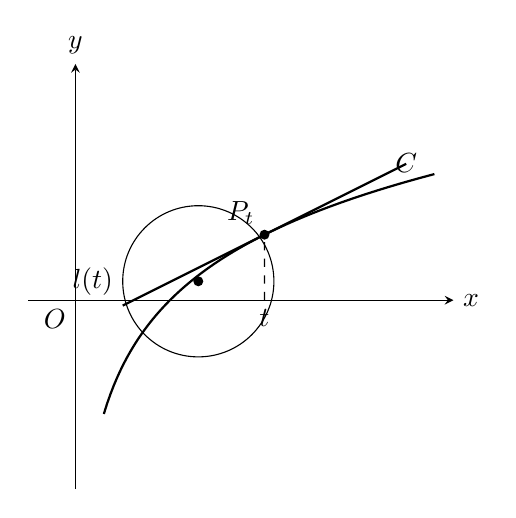
\begin{tikzpicture}[scale=1.2, >=stealth]
  \draw[->] (-0.5,0) -- (4,0) node[right] {$x$};
  \draw[->] (0,-2) -- (0,2.5) node[above] {$y$};
  \node[below left] at (0,0) {$O$};

  % Curve y = ln(x)
  \draw[thick, domain=0.3:3.8, samples=100] plot (\x, {ln(\x)});
  \node[above] at (3.5, {ln(3.5)}) {$C$};

  % Point P_t
  \coordinate (Pt) at (2, {ln(2)});
  \fill (Pt) circle (1.5pt) node[above left] {$P_t$};
  \draw[dashed] (2,0) -- (Pt) node[pos=0, below] {$t$};

  % Tangent line l(t)
  \draw[thick, domain=0.5:3.5] plot (\x, {ln(2) + 0.5*(\x - 2)});
  \node[above left] at (0.5, {ln(2) + 0.5*(0.5 - 2)}) {$l(t)$};

  % Circle touching line and passing through Pt
  \draw (1.3, 0.2) circle (0.8);
  \fill (1.3, 0.2) circle (1.5pt);
\end{tikzpicture}
\end{center}

\subsection*{第3問}

\begin{tcolorbox}[title=整関数と割り切れに関するメモ]
\begin{itemize}
    \item $[ \text{整関数} ]$\\
    任意の $n$ 次整関数は
    \[
    f(x) = \sum_{k=0}^n f_k(x) a_k \quad \left( f_k(x) = (x+k)(x+k-1) \dots (x+1) x \right)
    \]
    と表せる.\\
    $f(x)$ が整関数 $\iff$ ある $k$ について $f(k) \in \mathbb{Z} \land f(x+1)-f(x)$ が整関数.
    \item $[ \text{割り切る} ]$\\
    $f(x)$ が $(x-\alpha)^k$ で割り切れるとき
    \[
    \iff f(\alpha) = f'(\alpha) = \dots = f^{(k-1)}(\alpha) = 0
    \]
    \item $[ \text{付} ]$\\
    $x-\alpha$ で割り切るための作業が出ている時, $t = x-\alpha$ とおいた方が見通しがよくなる.
\end{itemize}
\end{tcolorbox}

[解] $f_k(x) = x^k - 1 - k(x-1)$ とおくと 任意の $n$ 次多項式 $g(x)$ は,
\[
g(x) = \sum_{k=2}^n a_k f_k(x) + a_1 x + a_0
\]
とおける.

(i) $g(x)$ が $(x-1)^2$ で割り切れるには, $g(1)=g'(1)=0$ が必要十分であるが, $f_k(1)=f'_k(1)=0$ から, この条件は
\[
\begin{cases} a_1 + a_0 = 0 \\ a_1 = 0 \end{cases} \iff a_1 = a_0 = 0
\]
より, この時,
\[
g(x) = \sum_{k=2}^n a_k f_k(x) \quad \text{の形で表せる.} \quad \dots \text{①}
\]
逆に, ①の時, $g(1)=g'(1)=0$ となり, 十分.
以上から示された.

(ii) $g(x)$ が $(x-1)^3$ で割り切れるには, $g(1)=g'(1)=g''(1)=0$ が必要十分である. $f_k(1)=f'_k(1)=0, f''_k(1)=k(k-1)$ から
この時,
\[
\begin{cases} a_1 = a_0 = 0 \\ \sum_{k=2}^n k(k-1) a_k = 0 \end{cases}
\]
だから, たしかに $g(x) = \sum_{k=2}^n a_k f_k(x)$ ($\sum_{k=2}^n \frac{k(k-1)}{2} a_k = 0$) を書けることが必要. 逆に, このように書ける時, 同様にして十分である.
以上から示された.

[別解] (1) 十分性について.
\[
f_k(x) = \{(x-1)+1\}^k - k(x-1) - 1
\]
を $x-1$ の整式とみると
\[
f_k(x) = (t+1)^k - kt - 1 \quad (t=x-1)
\]
の 1 次以下の部分は $0$ だから, $f_k(x)$ は $(x-1)^2$ で割り切れる. よって, 十分.

・必要性
$n=1,2$ の時自明. $n < m$ の時, 「$(x-1)^2$ で割り切れる $g(x)$ は $\sum_{k=2}^n a_k f_k(x)$ の形で表せる」が真とする. $m+1$ 次の $g(x)$ は $m$ 次以下の整式 $h(x)$ として
\[
g(x) = a_m f_m(x) + h(x)
\]
と表せる. この時, $f_m(x), g(x)$ が共に $(x-1)^2$ で割り切れるので, $h(x)$ もそうである. よって仮定から示された.

(2) より, $f_k(x) = \sum_{i=2}^k {}_k\mathrm{C}_i (x-1)^i$ だから,
\[
\sum_{k=2}^n a_k f_k(x) = \sum_{k=2}^n a_k \left[ \sum_{i=2}^k {}_k\mathrm{C}_i (x-1)^i \right]
\]
で, これを $(x-1)^3$ でわったあまりは,
\[
\sum_{k=2}^n a_k {}_k\mathrm{C}_2 (x-1)^2
\]
だから, 示すべきことは明らか.

\subsection*{第4問}

[解] $z=k$ ($0 \le k \le \frac{\sqrt{3}}{4}$) で切ると, 断面積は右下図. したがって, この面での面積 $S(k)$ として
\[
S(k) = \pi \left[ \frac{1}{2} \left(1 - \frac{4\sqrt{3}}{3} k\right) \right]^2 = \frac{\pi}{4} \left( 1 - \frac{4\sqrt{3}}{3} k \right)^2
\]
だから,
\begin{align*}
V &= \int_0^{\sqrt{3}/4} S(k) \, dk \\
&= \frac{\pi}{4} \int_0^{\sqrt{3}/4} \left( 1 - \frac{4\sqrt{3}}{3} k \right)^2 \, dk \\
&= \frac{\pi}{4} \left[ -\frac{\sqrt{3}}{12} \left( \frac{4\sqrt{3}}{3} k - 1 \right)^3 \right]_0^{\sqrt{3}/4} \\
&= \frac{\sqrt{3}\pi}{48}
\end{align*}

(問題文 点 $R(\frac{1}{4}, 0, \frac{\sqrt{3}}{4})$ ?)

\begin{center}
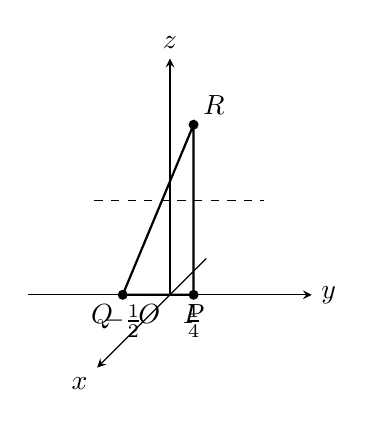
\begin{tikzpicture}[scale=1.2, >=stealth]
  \draw[->] (-1.5,0,0) -- (1.5,0,0) node[right] {$y$};
  \draw[->] (0,0,0) -- (0,2.5,0) node[above] {$z$};
  \draw[->] (0,0,-1) -- (0,0,2) node[below left] {$x$};
  \node[below left] at (0,0,0) {$O$};

  % Pyramid vertices P, Q, R
  \coordinate (P) at (0.25,0,0);
  \coordinate (Q) at (-0.5,0,0);
  \coordinate (R) at (0.25, 1.8, 0);

  \draw[thick] (P) -- (Q) -- (R) -- cycle;
  \fill (P) circle (1.5pt) node[below] {$P$};
  \fill (Q) circle (1.5pt) node[below left] {$Q$};
  \fill (R) circle (1.5pt) node[above right] {$R$};
  
  \node[below] at (0.25,0) {$\frac{1}{4}$};
  \node[below] at (-0.5,0) {$-\frac{1}{2}$};

  % Cross-section level z = k
  \draw[dashed] (-0.8, 1.0, 0) -- (1.0, 1.0, 0);
\end{tikzpicture}
\qquad
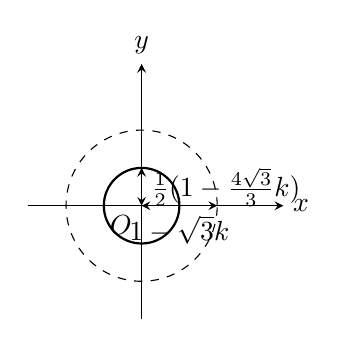
\begin{tikzpicture}[scale=1.2, >=stealth]
  \draw[->] (-1.2,0) -- (1.5,0) node[right] {$x$};
  \draw[->] (0,-1.2) -- (0,1.5) node[above] {$y$};
  \node[below left] at (0,0) {$O$};

  \draw[dashed] (0,0) circle (0.8);
  \draw[thick] (0,0) circle (0.4);

  \draw[<->] (0,0) -- (0,0.4) node[midway, right] {$\frac{1}{2}(1-\frac{4\sqrt{3}}{3}k)$};
  \draw[<->] (0,0) -- (0.8,0) node[midway, below] {$1-\sqrt{3}k$};
\end{tikzpicture}
\end{center}

\subsection*{第5問}

[解] 第 $n$ 世代に 1 個あるのは, 常に 1 個ずつの個体をのこす時で,
\[
P_n(1) = p^n \quad (1 \text{以下にも } z \ge 0 \text{ に拡張する})
\]

第 $n$ 世代に 2 個とするのは, 第 $m$ 世代になった時に ($m=1, 2, \dots, n$) 1 個から 2 個になる. この時第 $n$ 世代に 2 個である確率は
\[
P_{m-1}(1) \cdot (1-p) \{ p^{n-m} \}^2
\]
だから, $m$ について足して,
\begin{align*}
P_n(2) &= \sum_{m=1}^n P_{m-1}(1) (1-p) p^{2n-2m} \\
&= \sum_{m=1}^n p^{m-1} (1-p) p^{2n-2m} \\
&= (1-p) p^{2n-1} \sum_{m=1}^n \left(\frac{1}{p}\right)^m \\
&= \frac{1}{p} \frac{1-(1/p)^n}{1-1/p} (1-p) p^{2n-1} \\
&= (1-p^n) p^{n-1}
\end{align*}

\begin{center}
\begin{tikzpicture}[scale=1.0, >=stealth]
  \node (o) at (0,0) {$o$};
  \node (m1) at (2,0.5) {$m-1$};
  \node (m) at (3.5,0.8) {$m$};
  \node (n1) at (5,1.2) {$n$};
  \node (n2) at (5,0.2) {$n$};

  \draw (o) -- (m1);
  \draw (m1) -- (m);
  \draw (m) -- (n1);
  \draw (m) -- (n2);

  \fill (o) circle (1.5pt);
  \fill (m1) circle (1.5pt);
  \fill (m) circle (1.5pt);
  \fill (n1) circle (1.5pt);
  \fill (n2) circle (1.5pt);
\end{tikzpicture}
\end{center}

さいごに, 第 $n$ 世代で 3 個となる時, 第 $m$ 世代の時にはじめて 2 個から 3 個となるような $m$ ($m=2, 3, \dots, n$) がある. このような確率は
\[
P_{m-1}(2) \cdot 2 \cdot p (1-p) \{ p^{n-m} \}^3 \quad (\text{※ 2個のうちどちらかが2個に分裂するか})
\]
\[
= 2(1-p^{m-1}) p^{m-2} \cdot p(1-p) p^{3n-3m} = 2(1-p) p^{3n-1} (1-p^{m-1}) p^{-2m}
\]
\[
= 2(1-p) p^{3n-1} (p^{-2m} - p^{-m-1})
\]
より, $n \ge 2$ に対して,
\[
P_n(3) = 2(1-p) p^{3n-1} \sum_{m=2}^n \left\{ \left(\frac{1}{p^2}\right)^m - \left(\frac{1}{p}\right)^{m+1} \right\} \quad \dots \text{①}
\]
ここで,
\[
\begin{cases}
\sum_{m=2}^n \left(\frac{1}{p^2}\right)^m = \frac{1}{p^4} \frac{1-(1/p^2)^{n-1}}{1-1/p^2} = \frac{1-(1/p^2)^{n-1}}{(p^2-1)p^2} \\
\sum_{m=2}^n \left(\frac{1}{p}\right)^{m+1} = \frac{1}{p^3} \frac{1-(1/p)^{n-1}}{1-1/p} = \frac{1-(1/p)^{n-1}}{(p-1)p^2}
\end{cases}
\]
を①に代入して
\begin{align*}
P_n(3) &= 2(1-p) p^{3n-1} \left[ \frac{1-(1/p^2)^{n-1}}{(p^2-1)p^2} - \frac{1-(1/p)^{n-1}}{(p-1)p^2} \right] \\
&= 2 p^{3n-3} \left[ 1 - (1/p)^{n-1} - \frac{1-(1/p^2)^{n-1}}{1+p} \right] \\
&= 2 \left[ p^{3n-3} - p^{2n-2} - \frac{p^{3n-3}-p^{n-1}}{1+p} \right] \\
&= \frac{2}{1+p} \left[ p^{3n-2} - (1+p) p^{2n-2} + p^{n-1} \right] \quad \dots \text{②}
\end{align*}

$n=1$ の時, $P_1(3)=0$ で, ②の表示で良い. よって
\[
P_n(3) = \frac{2}{1+p} \left[ p^{3n-2} - (1+p) p^{2n-2} + p^{n-1} \right]
\]

\subsection*{第6問}

[解] $y=x^2$ を $P(a,b)$ に関して対称移動すると, $(2b-y) = (2a-x)^2$ にうつるから
\[
U: y \le -(x-2a)^2 + 2b \equiv f(x)
\]
となる. $D \cap U \neq \phi, E \cap U \neq \phi$ から, $y=f(x)$ と $y=x^2$, $y=f(x)$ と $y=(x-4)^2$ は共有点を持つ.
さらに $D \cap E \cap U = \phi$ から, (*)の条件は
\[
\begin{cases}
\text{「 } y=f(x) \text{ と } y=x^2 \text{ が } x < 2 \text{ に共有点を持つ 」} \quad \dots \text{①} \\
\text{かつ 「 } y=f(x) \text{ と } y=(x-4)^2 \text{ が } 2 < x \text{ に共有点を持つ 」} \quad \dots \text{②}
\end{cases}
\]
である.

①について $x^2 + (x-2a)^2 - 2b = 0$ が $x < 2$ に解を持つ
②について $(x-4)^2 + (x-2a)^2 - 2b = 0$ が $2 < x$ に解を持つ

ここに注意し, $g(x) = x^2 + (x-2a)^2 - 2b$, $h(x) = (x-4)^2 + (x-2a)^2 - 2b$ とおく.

①について
$g(x) = 2x^2 - 4ax + 4a^2 - 2b$ で, $g(x)=0$ の判別式 $D_1$ として
\[
\begin{cases}
D_1/4 \ge 0 \\
\text{軸} : a < 2 \\
\text{端} : g(2) > 0
\end{cases}
\iff
\begin{cases}
(2a)^2 - 2(4a^2 - 2b) \ge 0 \\
a < 2 \\
2a^2 - 4a + 4 - b > 0
\end{cases}
\iff
\begin{cases}
b \ge a^2 \\
a < 2 \\
b < 2a^2 - 4a + 4
\end{cases}
\quad \dots \text{③}
\]

②について
$h(x) = 2x^2 - (4a+8)x + 4a^2 + 16 - 2b$ で, $h(x)=0$ の判別式 $D_2$ として
\[
\begin{cases}
D_2/4 \ge 0 \\
\text{軸} : 2 < a+2 \\
\text{端} : h(2) > 0
\end{cases}
\iff
\begin{cases}
(2a+4)^2 - 2(4a^2 + 16 - 2b) \ge 0 \\
0 < a \\
2a^2 - 4a + 4 - b > 0
\end{cases}
\iff
\begin{cases}
b \ge a^2 - 4a + 4 \\
0 < a \\
b < 2a^2 - 4a + 4
\end{cases}
\quad \dots \text{④}
\]

以上から, ③かつ④が求める条件で, 図示して下図斜線部 (境界は実線のみ含む)

＜条件＞
\[
\begin{cases}
a^2 \le b < 2a^2 - 4a + 4 \quad \text{かつ} \\
a^2 - 4a + 4 \le b < 2a^2 - 4a + 4 \quad \text{かつ} \\
0 < a < 2
\end{cases}
\]

\begin{center}
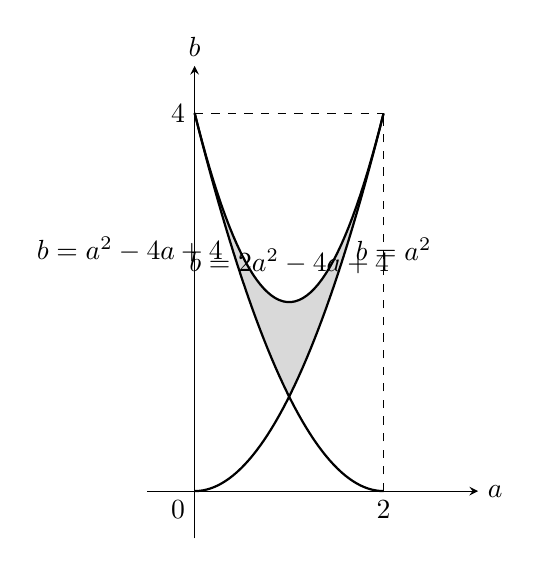
\begin{tikzpicture}[scale=1.2, >=stealth]
  \draw[->] (-0.5,0) -- (3,0) node[right] {$a$};
  \draw[->] (0,-0.5) -- (0,4.5) node[above] {$b$};
  \node[below left] at (0,0) {$0$};

  % Key points
  \node[below] at (2,0) {$2$};
  \draw[dashed] (2,0) -- (2,4);
  \node[left] at (0,4) {$4$};
  \draw[dashed] (0,4) -- (2,4);

  % Shading the region
  \fill[gray!30, domain=0:1, samples=50] plot (\x, {(\x-2)^2}) -- plot[domain=1:0] (\x, {2*\x*\x - 4*\x + 4}) -- cycle;
  \fill[gray!30, domain=1:2, samples=50] plot (\x, {\x*\x}) -- plot[domain=2:1] (\x, {2*\x*\x - 4*\x + 4}) -- cycle;

  % Curves
  \draw[thick, domain=0:2, samples=50] plot (\x, {\x*\x});
  \node[right] at (1.6, 2.56) {$b = a^2$};

  \draw[thick, domain=0:2, samples=50] plot (\x, {(\x-2)^2});
  \node[left] at (0.4, 2.56) {$b = a^2 - 4a + 4$};

  \draw[thick, domain=0:2, samples=50] plot (\x, {2*\x*\x - 4*\x + 4});
  \node[above] at (1, 2.2) {$b = 2a^2 - 4a + 4$};
\end{tikzpicture}
\end{center}

\end{document}
